
\begin{name}
	{\tenchude}
	{TOÁN 10}
	{LỚP TOÁN THẦY PHÁT}
	{Thời gian: 30 phút - Không kể thời gian phát đề}
\end{name}
\setcounter{page}{1}
\TN
\Opensolutionfile{ans}[ans/ansBONPA-0D1-OnChuong-De1]
\begin{ex}%[0D1N1-1]
Phát biểu nào sau đây là mệnh đề?
\choice
{\True Thầy Phát không quá 30 tuổi}
{Bạn có thích môn Toán không?}
{Cấm học sinh quay cóp trong kiểm tra}
{Ê, chọn câu C đi.}
\loigiai{
\lq\lq Thầy Phát không quá 30 tuổi\rq\rq\, là một mệnh đề vì đây là một câu khẳng định sai.
}
\end{ex}

\begin{ex}%[Thi GHK1, Lê Quí Đôn - Ninh Thuận, 2018]%[Ngụy Như Thái, EX-DT-10&11]%[0D1N1-2]
Cho mệnh đề chứa biến $P\left(n\right)\colon \lq\lq n^3+1 $ chia hết cho $3$\rq\rq. Khẳng định nào sau đây \textbf{đúng}?
\choice
{\True$ P(2)$ đúng, $P(5)$ đúng}
{$P(2)$ sai, $P(5)$ sai}
{$P(2)$ đúng, $P(5)$ sai}
{$P(2)$ sai, $P(5)$ đúng}
\loigiai{
Ta có $P\left(2\right)\colon \lq\lq 2^3+1 $ chia hết cho $3$\rq\rq\;là mệnh đề đúng.\\
$P\left(5\right)\colon \lq\lq 5^3+1 $ chia hết cho $3$\rq\rq \;là mệnh đề đúng.}
\end{ex}

\begin{ex}%[Lê Quốc Dũng-Dự Án TEX TLDH5]%[0D1N1-3]
Cho mệnh đề \lq\lq  $\forall x\in \mathbb{R},\, x^2-x+7 < 0$ \rq\rq . Mệnh đề nào là mệnh đề phủ định của mệnh đề trên?
\choice
{\True $\exists x\in \mathbb{R},\ x^2-x+7\ge 0$}
{$\forall x\in \mathbb{R},\, x^2-x+7>0$}
{$\forall x\in \mathbb{R},\, x^2-x+7 < 0$}
{$\exists x\in \mathbb{R},\, x^2-x+7 > 0$}
\loigiai{
}
\end{ex}

\begin{ex}%[05]%[Nguyễn Diệu Linh]%[0D1H1-4]
Trong các mệnh đề sau, mệnh đề nào có mệnh đề đảo \textbf{đúng}?
\choice
{Nếu số nguyên $n$ có chữ số tận cùng là $5$ thì số nguyên $n$ chia hết cho $5$}
{\True Nếu tứ giác $ABCD$ có hai đường chéo cắt nhau tại trung điểm mỗi đường thì tứ giác $ABCD$ là hình bình hành}
{Nếu tứ giác $ABCD$ là hình chữ nhật thì tứ giác $ABCD$ có hai đường chéo bằng nhau}
{Nếu tứ giác $ABCD$ là hình thoi thì tứ giác $ABCD$ có hai đường chéo vuông góc với nhau}
\loigiai
{
\begin{itemize}
\item Xét mệnh đề đảo của mệnh đề $\lq\lq $Nếu số nguyên $n$ có chữ số tận cùng là $5$ thì số nguyên $n$ chia hết cho $5"$: $\lq\lq $Nếu số nguyên $n$ chia hết cho $5$ thì số nguyên $n$ có chữ số tận cùng là $5"$. Mệnh đề này sai vì số nguyên $n$ cũng có thể có chữ số tận cùng là $0$ .
\item Xét mệnh đề đảo của mệnh đề $\lq\lq $Nếu tứ giác $ABCD$ có hai đường chéo cắt nhau tại trung điểm mỗi đường thì tứ giác $ABCD$ là hình bình hành$"$: $\lq\lq $Nếu tứ giác $ABCD$ là hình bình hành thì tứ giác $ABCD$ có hai đường chéo cắt nhau tại trung điểm mỗi đường$"$. Mệnh đề này đúng.
\item Xét mệnh đề đảo của mệnh đề $\lq\lq $Nếu tứ giác $ABCD$ là hình chữ nhật thì tứ giác $ABCD$ có hai đường chéo bằng nhau$"$: $\lq\lq $Nếu tứ giác $ABCD$ có hai đường chéo bằng nhau thì tứ giác $ABCD$ là hình chữ nhất$"$. Mệnh đề này sai vì hình thang cân cũng có hai đường chéo bằng nhau, nhưng không là hình chữ nhật.
\item Xét mệnh đề đảo của mệnh đề $\lq\lq $Nếu tứ giác $ABCD$ là hình thoi thì tứ giác $ABCD$ có hai đường chéo vuông góc$"$: $\lq\lq $Nếu tứ giác $ABCD$ có hai đường chéo vuông góc thì tứ giác $ABCD$ là hình thoi$"$. Mệnh đề này sai.

\end{itemize}
}
\end{ex}

\begin{ex}%[0D1H2-1]
Tập hợp nào sau đây là tập hợp rỗng?
\choice
{$\mathrm{A}= \left\{x \in \mathbb{R} \vert x^2 - x = 0 \right\}$}
{\True $\mathrm{B}= \left\{x \in \mathbb{Q} \vert x^2 = 2 \right\}$}
{$\mathrm{C}= \left\{x \in \mathbb{R} \vert x^2 - 1 = 0 \right\}$}
{$\mathrm{D}= \left\{x \in \mathbb{Z} \vert 0 < x < 4 \right\}$}
\loigiai
{
$x^2 - x = 0 \Leftrightarrow \hoac{& x = 0 \\& x = 1}$. Cho nên $\mathrm{A} = \{0;1\}$.\\
$\heva{& x \in \mathbb{Q} \\& x^2 = 2} \Leftrightarrow \heva{& x \in \mathbb{Q} \\& x = \pm \sqrt{2}}$ (vô nghiệm). Cho nên $\mathrm{B} = \varnothing$.\\
$x^2 - 1 = 0 \Leftrightarrow x = \pm 1$. Cho nên $\mathrm{C} = \{-1;1\}$.\\
$\heva{& x \in \mathbb{Z} \\& 0 < x < 4} \Leftrightarrow x \in \{1;2;3\}$. Cho nên $\mathrm{D} = \{1;2;3\}$.
}
\end{ex}

\begin{ex}%[Nguyễn Trần Phong, dự án 01YTB]%[0D1N3-1]
Cho hai tập hợp $A = \left\{ -2, 0, 1, 4, 6, 8 \right\}$ và $B =\left\{-2, 1, 4, 5, 6, 7\right\}$. Tìm tập hợp $A \cap B$.
\choice
{\True $\left\{ -2, 1, 4, 6\right\}$}
{$\left\{-2, 0, 1, 4, 5, 6, 7, 8\right\}$}
{$\left\{0, 1, 8\right\}$}
{$\left\{1, 4, 7\right\}$}
\loigiai{
Ta có	$A \cap B=\left\{ -2, 1, 4, 6\right\}$.
}
\end{ex}
\Closesolutionfile{ans}
\TNTF
% \setcounter{ex}{0}
\Opensolutionfile{ans}[ans/ansDS-0D1-OnChuong-De1]
\begin{ex}%[Mức độ 2]%[Trần Bá Huy, dự án 24-25 giảng 10,11]%[0D1H1-5]
Cho mệnh đề chứa biến $P(n):$ \lq\lq $n^2-2$ là số lẻ\rq\rq\, với $n\in\mathbb{N}$. Cho tập hợp\\ $A=\{n\in \mathbb{N} \mid n^2+2 \text{ là số lẻ và } n\ge6 \}$. Xác định tính đúng sai của các khẳng định sau.
\choiceTF
{$P(n)$ là một mệnh đề}
{\lq\lq $\forall n\in\mathbb{N},\, P(n)$\rq\rq\, không là mệnh đề}
{\True $P(2)$ là mệnh đề sai}
{Tập hợp $A$ có nhiều hơn $4$ phần tử}
\loigiai{
\begin{itemchoice}
\itemch $P(n)$ là mệnh đề chứa biến chứ không phải là mệnh đề.
\itemch $\forall n\in\mathbb{N},\, P(n)$ là một mệnh đề chứa kí hiệu $\forall$.
\itemch Với $n=2$, $n^2-2=2$ là số chẵn nên $P(2)$ là mệnh đề sai.
\itemch $n^2-2$ là số lẻ nên $n^2$ là số lẻ. Suy ra $n$ là số lẻ. Do đó $A=\{1;3;5\}$ nên có $3$ phần tử.
\end{itemchoice}
}
\end{ex}
\Closesolutionfile{ans}
\TNSA
% \setcounter{ex}{0}
\Opensolutionfile{ans}[ans/ansTLN-0D1-OnChuong-De1]
\begin{ex}%[Mức độ 2]%[Trần Bá Huy, dự án 24-25 giảng 10,11]%[0D1H1-5]
Biết rằng \lq\lq $\exists n\in\mathbb{N},\, 2n+3$ là số chính phương\rq\rq\, là mệnh đề đúng. Tức là tồn tại $n_0\in \mathbb{N}$ sao cho \lq\lq $2n_0+3$ là số chính phương\rq\rq\, là mệnh đề đúng. Tìm tích tất cả các giá trị của $n_0\in [0;15]$ thỏa mãn.
\shortans{$33$}
\loigiai{
Bằng cách thử trực tiếp, ta thấy $2n_0+3$ là số chính phương khi $n_0\in \{3;11\}$.\\
Vậy tích tất cả các giá trị $n_0$ thỏa mãn bằng $33$.
}
\end{ex}

\begin{ex}%[0D1H2-3]
Cho hai tập hợp $A=(-\infty ; 3]$ và $B=[-1 ; 5)$. Tập hợp $B \setminus A$ chứa bao nhiêu số nguyên.

\shortans{1}
\loigiai{
Tập hợp $B \setminus A=(3;5)$ chứa $1$ số nguyên.
}
\end{ex}

\begin{ex}%[0D1V3-5]
Lớp 10C14 có $45$ học sinh chuẩn bị cho hội diễn văn nghệ chào mừng ngày nhà giáo Việt Nam 20/11. Trong danh sách đăng kí tham gia tiết mục nhảy Flashmob và tiết mục hát, có $35$ học sinh tham gia tiết mục nhảy Flashmob, $10$ học sinh tham gia cả hai tiết mục. Hỏi có bao nhiêu học sinh trong lớp tham gia tiết mục hát? Biết rằng lớp 10C14 có bạn Kiệt, Hạ, Toàn, Thiện bị khuyết tật hòa nhập nên không tham gia tiết mục nào.
\shortans{16}
\loigiai{
\immini[thm]{Kí hiệu $A$ là tập hợp học sinh tham gia tiết mục nhảy Flashmob, $B$ là tập hợp học sinh tham gia tiết mục hát, $E$ là tập hợp học sinh trong lớp. Ta có thể biểu diễn ba tập hợp đó bằng biểu đồ Ven như hình bên.}
{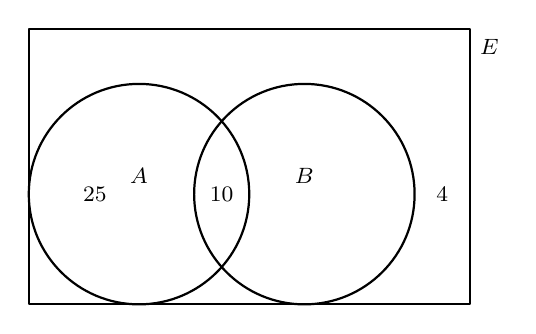
\begin{tikzpicture}[scale=.7, font=\footnotesize, line join=round, line cap=round, >=stealth]
% Draw the rectangle (universal set E)
\draw[thick] (-3,-2) rectangle (5,3) node[below right] {$E$};

% Draw the circles (sets A and B)
\draw[thick] (-1,0) circle (2) node[above] {$A$};
\draw[thick] (2,0) circle (2) node[above] {$B$};

% Add numbers inside the regions
\node at (-1.8,0) {25}; % Region in A only
\node at (0.5,0) {10}; % Overlap (A ∩ B)
\node at (4.5,0) {4};  % Region in B only
\end{tikzpicture}}
Khi đó, $A\cap B$ là tập hợp học sinh tham gia cả hai tiết mục. Số phần tử của tập hợp $A$ là $35$, số phần tử của tập hợp $A\cap B$ là $10$, số phần tử của tập hợp $E$ là $45$.\\
Số học sinh tham gia ít nhất một trong hai tiết mục là $45-4=41$ (học sinh).\\
Số học sinh tham gia tiết mục hát mà không tham gia tiết mục nhảy Flashmob là \break$41-35=6$ (học sinh).\\
Số học sinh tham gia tiết mục hát là $6+10=16$ (học sinh).
}
\end{ex}
\Closesolutionfile{ans}
\TL
\begin{ex}%[0D1H3-4]
Cho tập $A=(-3 ; 0]$ và $B=[-1 ; 1)$. Xác định các tập hợp sau và biểu diễn chúng lên trục số $A \cup B$, $A \cap B$, $A \setminus B$ và $\mathrm{C}_{\mathrm{R}} B$.
\loigiai{
\begin{itemize}
\item $A \cup B=(-3;1)$.
\item $A \cap B=[-1;0]$.
\item $A \setminus B=(-3;-1)$.
\item $\mathrm{C}_{\mathrm{R}} B=(-\infty;-1)\cup [1;+\infty)$.
\end{itemize}
}
\end{ex}

\begin{ex}%[Dự án Giảng 10-11 Nhóm Toán & LaTex, Lê Minh Thiện Anh]%[0D1H3-5]
Lớp 10C có $45$ học sinh, trong đó có $18$ học sinh tham gia cuộc thi vẽ đồ họa trên máy tính, $24$ học sinh tham gia cuộc thi tin học văn phòng cấp trường và $9$ học sinh không tham gia cả hai cuộc thi này. Hỏi có bao nhiêu học sinh của lớp 10C tham gia đồng thời hai cuộc thi?
\loigiai{
Kí hiệu $A$ và $B$ lần lượt là tập hợp các học sinh của lớp 10C dự thi vẽ đồ họa trên máy tính và dự thi tin học văn phòng. Khi đó, $A\cap B$ là tập hợp các học sinh của lớp dự thi cả hai môn; $A\cup B$ là tập hợp các học sinh của lớp dự thi ít nhất một trong hai môn.\\
Theo giả thiết, ta có $n(A)=18$, $n(B)=24$ và $n(A\cup B)=45-9=36$.\\
Ta có $n(A\cup B)=n(A)+n(B)-n(A\cap B)$.\\
Suy ra $n(A\cap B)=n(A)+n(B)-n(A\cup B)=18+24-36=6$.\\
Vậy lớp 10C có $6$ học sinh tham gia đồng thời cả hai cuộc thi.
}
\end{ex}
\dongcham{18}